% 验证案例自己的组件；不修改正式译稿。
% 缩进在当前字号选定后设置，因此测量与输出会执行同一段代码。
\newcommand{\ENIndent}{\setlength{\parindent}{1.5em}}
\newcommand{\ZHIndent}{\setlength{\parindent}{2em}}
\newcommand{\PDFNoIndent}{\setlength{\parindent}{0pt}\noindent}
\newcounter{ProbeRuns}\globalcounter{ProbeRuns}
\newcommand{\ProbeOnce}{\stepcounter{ProbeRuns}}
\newcommand{\DemoHeading}[3]{%
  \ifx#1\centering \phead[center]{#2}{#3}%
  \else \phead[left]{#2}{#3}\fi}

\ExplSyntaxOn
\NewDocumentEnvironment{demopair}{m m +b}
 {\str_if_eq:nnTF {#1}{fixed}
  {\begin{textpair}[id=#2,mode=fixed]#3\end{textpair}}
  {\begin{textpair}[id=#2]#3\end{textpair}}}{}
\ExplSyntaxOff
\SourceHasTeXtrue
\begin{document}
\begin{pair}
\noindent{\centering\DocumentTitleStyle Bilingual Layout Validation\par}
\switchcolumn
\noindent{\centering\DocumentTitleStyle 双栏翻译排版验证案例\par}
\end{pair}
\DemoHeading{\centering}{1 Centered heading}{1 居中标题}
\begin{demopair}{auto}{PLAIN}
\ENIndent\noindent This synthetic document tests the components needed by a reusable bilingual translation template. It includes a reused raster figure, a translated table, genuine footnotes, a long equation, and a theorem that continues across pages. Ordinary paragraphs can choose a Chinese font size automatically, whereas blocks with side effects must be rendered exactly once. The visual and structural checks complement successful compilation.
\switchcolumn
\ZHIndent 这个独立案例验证双栏翻译模板：图片复用、表格翻译、正式脚注、长公式及跨页定理。普通中文段落允许自动选择字号，含副作用的块只排版一次。
\end{demopair}
\DemoHeading{\raggedright}{2 Figure and translated table}{2 图片与双栏表格}
\begin{demopair}{fixed}{FIGURE}
\hypertarget{figure:1:en}{}\noindent\begin{minipage}{\linewidth}\centering
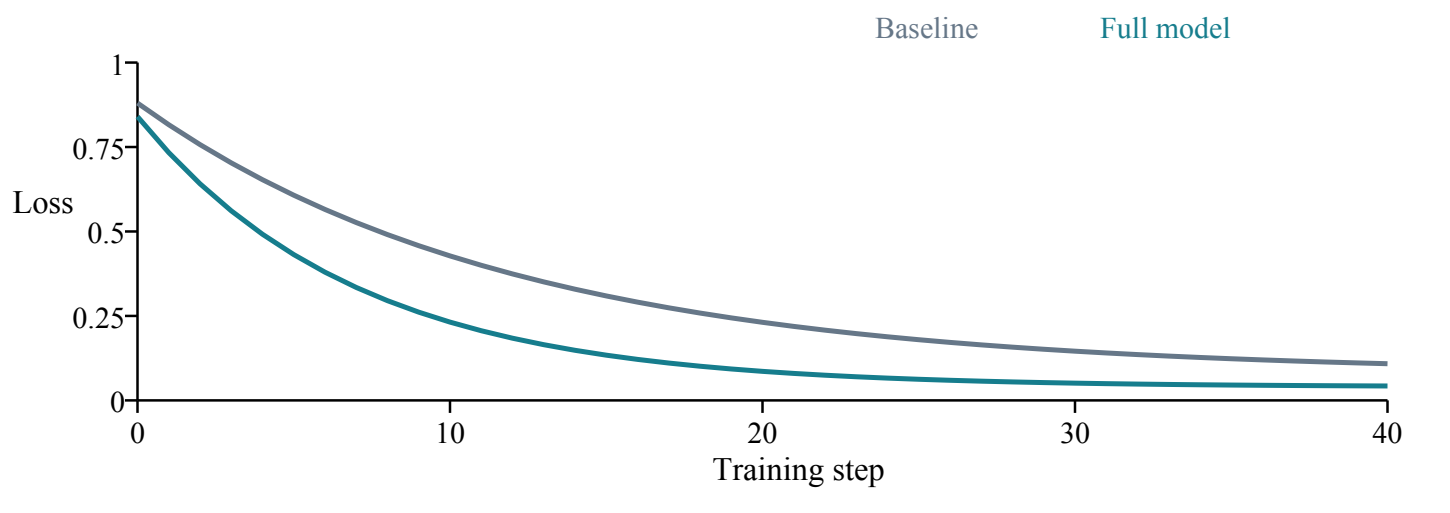
\includegraphics[width=.86\linewidth]{test-figure.png}\par
\textbf{Figure 1.} Two synthetic learning curves; the image text is retained.\par
\end{minipage}
\switchcolumn
\hypertarget{figure:1:zh}{}\noindent\begin{minipage}{\linewidth}\centering
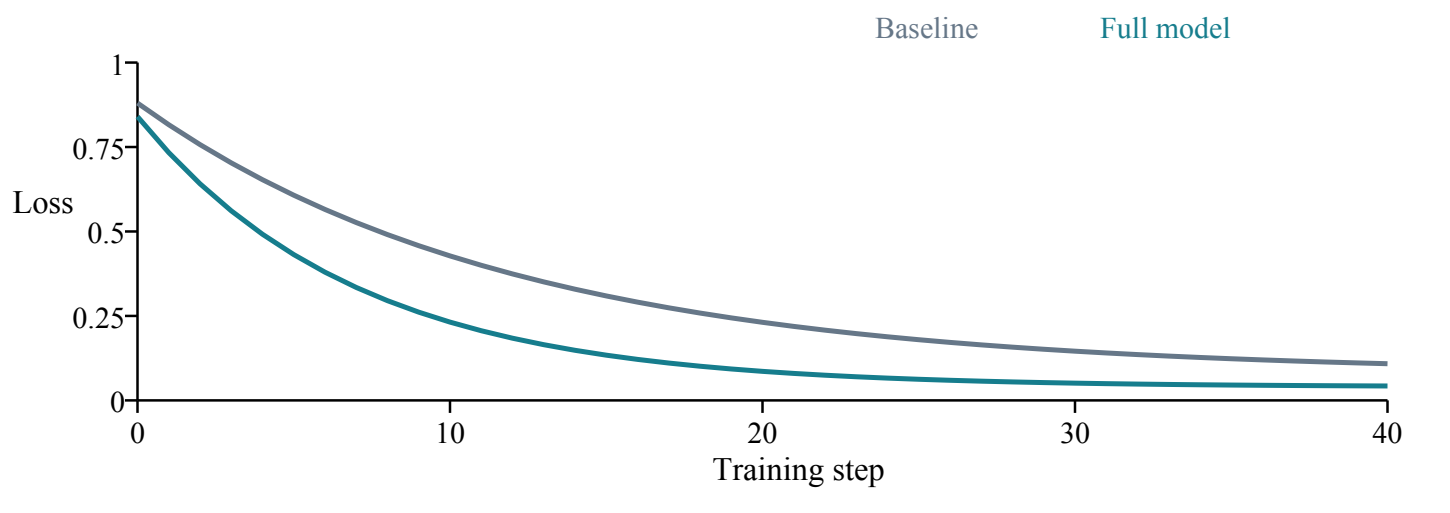
\includegraphics[width=.86\linewidth]{test-figure.png}\par
\textbf{图 1.} 两条模拟学习曲线；图片内的英文保持原样。\par
\end{minipage}
\end{demopair}
\begin{demopair}{fixed}{TABLE}
\hypertarget{table:1:en}{}\noindent\begin{minipage}{\linewidth}\centering
\textbf{Table 1.} Synthetic results\par\medskip
\begin{tabular}{@{}lcc@{}}\toprule Model & Samples & Error\\\midrule Baseline & 100 & 0.120\\ Ablation & 200 & 0.081\\ Full model & 400 & 0.043\\\bottomrule\end{tabular}\par
\end{minipage}
\switchcolumn
\hypertarget{table:1:zh}{}\noindent\begin{minipage}{\linewidth}\centering
\textbf{表 1.} 模拟结果\par\medskip
\begin{tabular}{@{}lcc@{}}\toprule 模型 & 样本数 & 误差\\\midrule 基准模型 & 100 & 0.120\\ 消融模型 & 200 & 0.081\\ 完整模型 & 400 & 0.043\\\bottomrule\end{tabular}\par
\end{minipage}
\end{demopair}
\DemoHeading{\raggedright}{3 Genuine footnotes}{3 正式脚注}
% 故意写 auto；组件会识别 footnote 与 label，并改用固定字号。
% 两栏复用原脚注编号 1；hyperref 为两次真实脚注分别生成目标。
\begin{demopair}{auto}{FOOTNOTE}
\ENIndent\noindent\ProbeOnce\phantomsection\label{fn:block:en}This paragraph carries one genuine footnote.\SourceFootnote{1}{English footnote payload: FOOTNOTE-EN-ONCE.} The callout retains source number 1.
\switchcolumn
\ZHIndent\ProbeOnce\phantomsection\label{fn:block:zh}这一段包含正式脚注。\SourceFootnote{1}{中文脚注只输出一次，标记为 FOOTNOTE-ZH-ONCE。} 脚注标记保留原编号 1。
\end{demopair}
\clearpage
\DemoHeading{\raggedright}{4 Independent long equation}{4 独立的长公式}
\begin{demopair}{auto}{REFS}
\ENIndent\noindent See \NumberedLink{figure:1:en}{Figure}{1}, \NumberedLink{table:1:en}{Table}{1}, and \NumberedLink{theorem:1:en}{Theorem}{1}. Equation (\hyperref[eq:long:en]{\ref*{eq:long:en}}) has three aligned lines and one source number. Its reference is resolved on the later compilation pass.
\switchcolumn
\ZHIndent 参见\NumberedLink{figure:1:zh}{图}{1}、\NumberedLink{table:1:zh}{表}{1}及\NumberedLink{theorem:1:zh}{定理}{1}。公式 (\hyperref[eq:long:zh]{\ref*{eq:long:zh}}) 分为三行，保留一个编号。
\end{demopair}
\begin{equationpair}\begin{equation}\begin{aligned}
\mathcal J(\theta)&=\frac1n\sum_{i=1}^n\|f_\theta(x_i)-y_i\|_2^2\\
&\quad+\lambda\sum_{\ell=1}^L\bigl(\|W_\ell\|_F^2+\|b_\ell\|_2^2\bigr)\\
&\quad+\mu\,\mathbb E_{x\sim\rho}\|\nabla_x f_\theta(x)\|_2^2.
\end{aligned}\tag{1}\label{eq:long:en}\end{equation}\switchcolumn\begin{equation}\begin{aligned}
\mathcal J(\theta)&=\frac1n\sum_{i=1}^n\|f_\theta(x_i)-y_i\|_2^2\\
&\quad+\lambda\sum_{\ell=1}^L\bigl(\|W_\ell\|_F^2+\|b_\ell\|_2^2\bigr)\\
&\quad+\mu\,\mathbb E_{x\sim\rho}\|\nabla_x f_\theta(x)\|_2^2.
\end{aligned}\tag{1}\label{eq:long:zh}\end{equation}\end{equationpair}
\begin{demopair}{auto}{LABEL}
\ENIndent\noindent\ProbeOnce\phantomsection\label{probe:label:en}A label and a custom counter call appear in this block. The direct label command must force the fixed route, so the custom call is executed once.
\switchcolumn
\ZHIndent\ProbeOnce\phantomsection\label{probe:label:zh}此块包含标签及自定义计数器调用。显式标签应使它采用固定路径，计数器只执行一次。
\end{demopair}
\begin{demopair}{auto}{COUNTER}
\ENIndent\noindent\stepcounter{ProbeRuns}This block uses a counter directly and must also bypass measurement.
\switchcolumn
\ZHIndent\stepcounter{ProbeRuns}此块直接递增计数器，也必须跳过试排。
\end{demopair}
\DemoHeading{\raggedright}{5 Source-dependent indentation}{5 两种输入的缩进规则}
\begin{demopair}{fixed}{HEADING-FIRST}
\ENIndent\noindent First heading paragraph: English starts without indentation; Chinese uses the fixed two-character indent for a TeX source.
\switchcolumn
\ZHIndent 标题后首段：英文不缩进，中文仍采用两个汉字宽度的固定缩进。
\end{demopair}
\begin{demopair}{auto}{TEX-INDENT}
\ENIndent A subsequent paragraph for a TeX source begins with an indentation of 1.5 em. The indentation is evaluated at the active font size. It is applied both during the trial measurement and in the final typeset paragraph. This controlled example gives enough lines to compare natural heights without modifying counters or generating targets.
\switchcolumn
\ZHIndent 有 TeX 原文时，中文普通段落首行固定缩进两个汉字宽度。缩进在选定中文字号后计算，试排和最终输出使用相同设置。
\end{demopair}
\SourceHasTeXfalse
\begin{demopair}{auto}{PDF-NOINDENT}
For a PDF-only source, both language columns start at the column edge. This block tests the explicit no-indentation exception. It remains eligible for automatic Chinese sizing because the content contains no footnotes, labels, counter operations, or targets.
\switchcolumn
只有 PDF 原文时，两栏普通段落均不缩进。本块仍可自动选择中文字号，因为内容不含脚注、标签、计数器或锚点。
\end{demopair}\SourceHasTeXtrue
\clearpage
\DemoHeading{\raggedright}{6 One theorem across pages}{6 一个 pair 内的跨页定理}
\begin{pair}[\StatementKeepLines]
\hypertarget{theorem:1:en}{}\phantomsection\label{cross:start:en}
\begin{formaltheoremen}{\StatementNumber{Theorem}{1}}
Let $x_1,\ldots,x_n$ be vectors in a normed space. The following repeated estimates form a pagination stress test; every stage uses the triangle inequality. The complete English statement remains in this formal environment and in one outer pair.

\ENIndent Stage 1. Each vector contributes at most its own norm to the norm of the sum. The estimate does not require an inner product, a finite-dimensional representation, or any assumption about the signs of coordinates. The intermediate partial sums can therefore be bounded using the same rule. This paragraph deliberately supplies enough explanatory text to test natural page breaks without boxing the theorem.
\begin{equation*}\Bigl\|\sum_{i=1}^n x_i\Bigr\|\leq\sum_{i=1}^n\|x_i\|.\end{equation*}

\ENIndent Stage 2. Each vector contributes at most its own norm to the norm of the sum. The estimate does not require an inner product, a finite-dimensional representation, or any assumption about the signs of coordinates. The intermediate partial sums can therefore be bounded using the same rule. This paragraph deliberately supplies enough explanatory text to test natural page breaks without boxing the theorem.
\begin{equation*}\Bigl\|\sum_{i=1}^n x_i\Bigr\|\leq\sum_{i=1}^n\|x_i\|.\end{equation*}

\ENIndent Stage 3. Each vector contributes at most its own norm to the norm of the sum. The estimate does not require an inner product, a finite-dimensional representation, or any assumption about the signs of coordinates. The intermediate partial sums can therefore be bounded using the same rule. This paragraph deliberately supplies enough explanatory text to test natural page breaks without boxing the theorem.
\begin{equation*}\Bigl\|\sum_{i=1}^n x_i\Bigr\|\leq\sum_{i=1}^n\|x_i\|.\end{equation*}

\ENIndent Stage 4. Each vector contributes at most its own norm to the norm of the sum. The estimate does not require an inner product, a finite-dimensional representation, or any assumption about the signs of coordinates. The intermediate partial sums can therefore be bounded using the same rule. This paragraph deliberately supplies enough explanatory text to test natural page breaks without boxing the theorem.
\begin{equation*}\Bigl\|\sum_{i=1}^n x_i\Bigr\|\leq\sum_{i=1}^n\|x_i\|.\end{equation*}

\ENIndent Stage 5. Each vector contributes at most its own norm to the norm of the sum. The estimate does not require an inner product, a finite-dimensional representation, or any assumption about the signs of coordinates. The intermediate partial sums can therefore be bounded using the same rule. This paragraph deliberately supplies enough explanatory text to test natural page breaks without boxing the theorem.
\begin{equation*}\Bigl\|\sum_{i=1}^n x_i\Bigr\|\leq\sum_{i=1}^n\|x_i\|.\end{equation*}

\ENIndent Stage 6. Each vector contributes at most its own norm to the norm of the sum. The estimate does not require an inner product, a finite-dimensional representation, or any assumption about the signs of coordinates. The intermediate partial sums can therefore be bounded using the same rule. This paragraph deliberately supplies enough explanatory text to test natural page breaks without boxing the theorem.
\begin{equation*}\Bigl\|\sum_{i=1}^n x_i\Bigr\|\leq\sum_{i=1}^n\|x_i\|.\end{equation*}

\ENIndent Stage 7. Each vector contributes at most its own norm to the norm of the sum. The estimate does not require an inner product, a finite-dimensional representation, or any assumption about the signs of coordinates. The intermediate partial sums can therefore be bounded using the same rule. This paragraph deliberately supplies enough explanatory text to test natural page breaks without boxing the theorem.
\begin{equation*}\Bigl\|\sum_{i=1}^n x_i\Bigr\|\leq\sum_{i=1}^n\|x_i\|.\end{equation*}

\ENIndent Stage 8. Each vector contributes at most its own norm to the norm of the sum. The estimate does not require an inner product, a finite-dimensional representation, or any assumption about the signs of coordinates. The intermediate partial sums can therefore be bounded using the same rule. This paragraph deliberately supplies enough explanatory text to test natural page breaks without boxing the theorem.
\begin{equation*}\Bigl\|\sum_{i=1}^n x_i\Bigr\|\leq\sum_{i=1}^n\|x_i\|.\end{equation*}

\begin{equation*}\Bigl\|\sum_{i=1}^n x_i\Bigr\|\leq\sum_{i=1}^n\|x_i\|.\end{equation*}\phantomsection\label{cross:end:en}
\end{formaltheoremen}
\switchcolumn
\hypertarget{theorem:1:zh}{}\phantomsection\label{cross:start:zh}
\begin{formaltheoremzh}{\StatementNumber{定理}{1}}
设 $x_1,\ldots,x_n$ 是赋范空间中的向量。下面重复应用三角不等式，构成跨页排版压力测试。完整中文陈述保留在同一个定理环境及外层 pair 内。

\ZHIndent 阶段 1。每个向量对向量和的范数的贡献，不超过它自身的范数。这一估计不需要内积、有限维表示，也不要求坐标具有特定符号。因此，各个中间部分和可以采用同样的规则估计。本段特意保留较完整的说明文字，检验自然分页；定理正文不装入不可分页的盒子。
\begin{equation*}\Bigl\|\sum_{i=1}^n x_i\Bigr\|\leq\sum_{i=1}^n\|x_i\|.\end{equation*}

\ZHIndent 阶段 2。每个向量对向量和的范数的贡献，不超过它自身的范数。这一估计不需要内积、有限维表示，也不要求坐标具有特定符号。因此，各个中间部分和可以采用同样的规则估计。本段特意保留较完整的说明文字，检验自然分页；定理正文不装入不可分页的盒子。
\begin{equation*}\Bigl\|\sum_{i=1}^n x_i\Bigr\|\leq\sum_{i=1}^n\|x_i\|.\end{equation*}

\ZHIndent 阶段 3。每个向量对向量和的范数的贡献，不超过它自身的范数。这一估计不需要内积、有限维表示，也不要求坐标具有特定符号。因此，各个中间部分和可以采用同样的规则估计。本段特意保留较完整的说明文字，检验自然分页；定理正文不装入不可分页的盒子。
\begin{equation*}\Bigl\|\sum_{i=1}^n x_i\Bigr\|\leq\sum_{i=1}^n\|x_i\|.\end{equation*}

\ZHIndent 阶段 4。每个向量对向量和的范数的贡献，不超过它自身的范数。这一估计不需要内积、有限维表示，也不要求坐标具有特定符号。因此，各个中间部分和可以采用同样的规则估计。本段特意保留较完整的说明文字，检验自然分页；定理正文不装入不可分页的盒子。
\begin{equation*}\Bigl\|\sum_{i=1}^n x_i\Bigr\|\leq\sum_{i=1}^n\|x_i\|.\end{equation*}

\ZHIndent 阶段 5。每个向量对向量和的范数的贡献，不超过它自身的范数。这一估计不需要内积、有限维表示，也不要求坐标具有特定符号。因此，各个中间部分和可以采用同样的规则估计。本段特意保留较完整的说明文字，检验自然分页；定理正文不装入不可分页的盒子。
\begin{equation*}\Bigl\|\sum_{i=1}^n x_i\Bigr\|\leq\sum_{i=1}^n\|x_i\|.\end{equation*}

\ZHIndent 阶段 6。每个向量对向量和的范数的贡献，不超过它自身的范数。这一估计不需要内积、有限维表示，也不要求坐标具有特定符号。因此，各个中间部分和可以采用同样的规则估计。本段特意保留较完整的说明文字，检验自然分页；定理正文不装入不可分页的盒子。
\begin{equation*}\Bigl\|\sum_{i=1}^n x_i\Bigr\|\leq\sum_{i=1}^n\|x_i\|.\end{equation*}

\ZHIndent 阶段 7。每个向量对向量和的范数的贡献，不超过它自身的范数。这一估计不需要内积、有限维表示，也不要求坐标具有特定符号。因此，各个中间部分和可以采用同样的规则估计。本段特意保留较完整的说明文字，检验自然分页；定理正文不装入不可分页的盒子。
\begin{equation*}\Bigl\|\sum_{i=1}^n x_i\Bigr\|\leq\sum_{i=1}^n\|x_i\|.\end{equation*}

\ZHIndent 阶段 8。每个向量对向量和的范数的贡献，不超过它自身的范数。这一估计不需要内积、有限维表示，也不要求坐标具有特定符号。因此，各个中间部分和可以采用同样的规则估计。本段特意保留较完整的说明文字，检验自然分页；定理正文不装入不可分页的盒子。
\begin{equation*}\Bigl\|\sum_{i=1}^n x_i\Bigr\|\leq\sum_{i=1}^n\|x_i\|.\end{equation*}

\begin{equation*}\Bigl\|\sum_{i=1}^n x_i\Bigr\|\leq\sum_{i=1}^n\|x_i\|.\end{equation*}\phantomsection\label{cross:end:zh}
\end{formaltheoremzh}
\end{pair}
\begin{pair}\noindent The final displayed estimate belongs to the theorem above. English statement pages: \pageref*{cross:start:en}--\pageref*{cross:end:en}.\switchcolumn\noindent 定理末尾公式仍属于上面的定理。中文陈述页码：\pageref*{cross:start:zh}--\pageref*{cross:end:zh}。\end{pair}
\typeout{VALIDATION-PROBE-RUNS=\arabic{ProbeRuns}}
\typeout{VALIDATION-HFOOTNOTE=\arabic{Hfootnote}}
\end{document}
